%--------------------------------------------------------------------%
%
% Berkas utama templat LaTeX.
%
% author Petra Barus, Peb Ruswono Aryan, Faris Rizki Ekananda
%
%--------------------------------------------------------------------%
%
% Berkas ini berisi struktur utama dokumen LaTeX yang akan dibuat.
%
%--------------------------------------------------------------------%
\documentclass[bahasa, 12pt, a4paper, onecolumn, oneside, final]{report}

%-------------------------------------------------------------------%
%
% Konfigurasi dokumen LaTeX untuk laporan tesis IF ITB
%
% @author Petra Novandi
%
%-------------------------------------------------------------------%
%
% Berkas asli berasal dari Steven Lolong
%
%-------------------------------------------------------------------%

% Ukuran kertas
\special{papersize=210mm,297mm}

% Setting margin
\usepackage[top=2cm,bottom=2cm,left=4cm,right=3cm]{geometry}

% Math package
\usepackage{mathptmx}

% 4th Sectioning
\newcommand{\subsubsubsection}[1]{\paragraph{#1}\mbox{}\\}
\usepackage{titlesec}

\titleformat{\subsubsubsection}
{\normalfont\normalsize\bfseries}{\theparagraph}{1em}{}
\titleformat*{\section}{\normalsize\bfseries}
\titleformat*{\subsection}{\normalsize\bfseries}
\titlespacing*{\subsubsubsection}
{0pt}{3.25ex plus 1ex minus .2ex}{1.5ex plus .2ex}

% Judul bahasa Indonesia
\usepackage[bahasa]{babel}

% Format citation
\usepackage[utf8]{inputenc}
\usepackage[style=apa,backend=biber]{biblatex}
\usepackage{longtable}
\usepackage{graphicx}
\usepackage{subfig}
\usepackage{titling}
\usepackage{booktabs}
\usepackage{tabularx}
\usepackage{blindtext}
\usepackage{sectsty}
\usepackage{chngcntr}
\usepackage{etoolbox}
\usepackage{array}
\usepackage{float}
\usepackage[hidelinks]{hyperref}       % Package untuk link di daftar isi. Ubah jadi \usepackage[hidelinks]{hyperref} apabila ingin menghilangkan kotak merah disekitar link
\usepackage{titlesec}       % Package Format judul
\usepackage{titletoc}       % Package Format judul di toc
\usepackage{tocbibind}      % Package untuk masukkan toc, lot, lof ke Daftar Isi
\usepackage{scrwfile}       % Package untuk membuat Daftar Lampiran dari toc
\usepackage{parskip}
\usepackage{afterpage}
\usepackage{relsize}
\usepackage{xcolor, colortbl}
\usepackage{setspace}
\usepackage{listings}
\usepackage{csquotes}
\usepackage{amsmath,amssymb,amsfonts}
\usepackage{multirow}

% Gantt chart
\usepackage{pgfgantt}
\usepackage{lipsum}

\graphicspath{{resources/}}   % letak direktori penyimpanan gambar

% Setting daftar lampiran
\newcommand*{\lopname}{DAFTAR LAMPIRAN}
\TOCclone[\lopname]{toc}{atoc}
\addtocontents{atoc}{\protect\value{tocdepth}=-1}
\newcommand\listofappendices{
  \cleardoublepage
  \phantomsection
  \listofatoc
  \addcontentsline{toc}{chapter}{\lopname}
}

\newcommand*\savedtocdepth{}
\AtBeginDocument{%
  \edef\savedtocdepth{\the\value{tocdepth}}%
}

\let\originalappendix\appendix
\renewcommand\appendix{%
  \originalappendix
  \cleardoublepage
  \addtocontents{toc}{\protect\value{tocdepth}=-1}%
  \addtocontents{atoc}{\protect\value{tocdepth}=\savedtocdepth}%

  \titlecontents{chapter}
    [0pt]
    {\bfseries}
    {Lampiran \thecontentslabel.\quad}
    {}
    {\hfill\contentspage}

  \titleformat{\chapter}[block]
    {\bfseries}
    {\chaptertitlename\ \thechapter.\quad}{0pt}
    {\bfseries}
}

% Hilangkan titik pada toc
\makeatletter
\renewcommand{\@dotsep}{1} 
\makeatother

% Setel title pada chapter-chapter di toc, lof, lot
\titlecontents{chapter}
  [0pt]
  {\bfseries}
  {\MakeUppercase{Bab} \thecontentslabel\quad\uppercase}
  {}
  {\mdseries\titlerule*[0.35em]{.}\bfseries\contentspage}
\titlecontents{figure}
  [0pt]
  {}
  {Gambar \thecontentslabel.\quad}
  {}
  {\mdseries\titlerule*[0.35em]{.}\bfseries\contentspage}
\titlecontents{table}
  [0pt]
  {}
  {Tabel \thecontentslabel.\quad}
  {}
  {\mdseries\titlerule*[0.35em]{.}\bfseries\contentspage}

% Masukin Daftar Pustaka ke toc
\let\originalprintbibliography\printbibliography
\renewcommand\printbibliography{%
  \phantomsection
  \cleardoublepage
  \originalprintbibliography
  \addcontentsline{toc}{chapter}{\bibname}
}

% Line satu setengah spasi
\renewcommand{\baselinestretch}{1.5}

% Setting judul
% \chapterfont{\centering \large}
\titleformat{\chapter}[display]
  {\Large\centering\bfseries}
  {\chaptertitlename\ \thechapter}{0pt}
    {\Large\bfseries\uppercase}

% Setting nomor pada subbsubsubbab
\setcounter{secnumdepth}{4}

\makeatletter

\makeatother

% Counter untuk figure dan table.
\counterwithin{figure}{chapter}
\counterwithin{table}{chapter}

% Define blank page
\newcommand*{\blankpage}{\afterpage{\null\newpage}}

% Translate autoref into Indonesian
\renewcommand*{\equationautorefname}{Persamaan}%
\renewcommand*{\footnoteautorefname}{catatan kaki}%
\renewcommand*{\itemautorefname}{item}%
\renewcommand*{\figureautorefname}{Gambar}%
\renewcommand*{\tableautorefname}{Tabel}%
\renewcommand*{\partautorefname}{Bagian}%
\renewcommand*{\appendixautorefname}{Lampiran}%
\renewcommand*{\chapterautorefname}{Bab}%
\renewcommand*{\sectionautorefname}{Subbab}%
\renewcommand*{\subsectionautorefname}{Subsubbab}%
\renewcommand*{\subsubsectionautorefname}{Subsubsubbab}%
\renewcommand*{\paragraphautorefname}{paragraf}%
\renewcommand*{\subparagraphautorefname}{subparagraf}%
\renewcommand*{\FancyVerbLineautorefname}{garis}%
\renewcommand*{\theoremautorefname}{Teorema}%
\renewcommand*{\pageautorefname}{halaman}%

% Format to ignore underflow hbadness
\hbadness=99999

% Reusable Metadata
\newcommand\authorname{Muhamad Aji Wibisono}
\newcommand\authornim{13521095}
\newcommand\tanggalpengesahan{xxxx 2025}

%--------------------------------------------------------------------%
%
% Hypenation untuk Bahasa Indonesia
%
% @author Petra Barus
%
%--------------------------------------------------------------------%
%
% Secara otomatis LaTeX dapat langsung memenggal kata dalam dokumen,
% tapi sering kali terdapat kesalahan dalam pemenggalan kata. Untuk
% memperbaiki kesalahan pemenggalan kata tertentu, cara pemenggalan
% kata tersebut dapat ditambahkan pada dokumen ini. Pemenggalan
% dilakukan dengan menambahkan karakter '-' pada suku kata yang
% perlu dipisahkan.
%
% Contoh pemenggalan kata 'analisa' dilakukan dengan 'a-na-li-sa'
%
%--------------------------------------------------------------------%

\hyphenation {
  % A
  %
  a-na-li-sa
  a-pli-ka-si
  a-lo-ka-si
  an-ta-ra
  ada-nya
  akan
  % B
  %
  be-be-ra-pa
  ber-ge-rak
  be-ri-kut
  ber-ko-mu-ni-ka-si
  buah
  Bouvet
  ber-fo-kus
  ber-fung-si
  ber-ja-lan
  % C
  %
  ca-ri
  con-strained
  Carzaniga
  cloud
  CloudFormation
  con-tai-ner
  ClusterIP
  % D
  %
  da-e-rah
  di-nya-ta-kan
  de-fi-ni-si
  di-bu-tuh-kan
  di-gu-na-kan
  di-tam-bah-kan-nya
  di-tem-pat-kan
  di-la-ku-kan
  de-ploy-ment
  di-kem-bang-kan
  di-im-ple-men-ta-si-kan
  de-activation
  da-pat
  di-ka-te-go-ri-kan
  de-ngan
  di-kem-bang-kan
  da-ta
  % E
  %
  e-ner-gi
  eks-klu-sif
  eks-ter-nal
  % F
  %
  fa-si-li-tas
  % G
  %
  ga-bung-an
  % H
  %
  ha-lang-an
  ha-sil
  hell
  % I
  % 
  i-nduk
  in-for-ma-si
  im-ple-men-tasi
  % J
  %
  % K
  %
  kom-po-si-si
  ka-re-na
  ke-sa-ba-ran-nya
  ka-me-ra
  kua-li-tas
  ke-na-ngan
  kom-plek-si-tas
  ke-ti-ka
  ke-le-bi-han-nya
  ke-gi-a-tan
  ko-mu-ni-ka-si
  ke-cil
  % L
  %
  la-ya-nan
  % M
  %
  me-ngu-ra-ngi
  meng-eva-lu-a-si
  me-nge-lo-la
  men-da-lam
  men-ja-lan-kan
  mak-si-mal
  me-nye-le-sai-kan
  me-ngunjungi
  men-du-kung
  me-nu-rut
  me-la-ku-kan
  mem-buat
  men-daftar-kan
  me-ngu-sul-kan
  me-mi-li-ki
  meng-gu-na-kan
  men-ja-di
  me-ru-pa-kan
  men-ja-ga
  me-mu-dah-kan
  me-ne-rus-
  mem-pro-ses
  % N
  %
  Na-mun
  % O
  %
  ob-so-lete
  or-kes-tra-si
  oto-ma-ti-sa-si
  % P
  %
  pro-vi-der
  pe-ru-sa-ha-an
  pe-rang-kat
  pro-ses
  plat-form
  pro-duk-si
  pe-ne-li-tian
  pe-ru-ba-han
  pa-ra-dig-ma
  pe-man-tau-an
  pe-ngum-pu-lan
  pa-ckage
  % Q
  %
  quality
  % R
  %
  re-source
  re-mote
  % S
  se-la-in
  stan-dar-di-sasi
  se-cu-ri-ty
  so-lu-si
  se-lu-ruh
  Soft-ware
  soft-ware
  se-buah
  se-ca-ra
  %
  % T
  % 
  ter-li-bat
  ter-pi-sah-kan
  ter-mi-nal
  ter-ba-tas
  % U
  %
  un-tuk
  % V
  %
  % W
  %
  % X
  %
  % Y
  % 
  % Z
  %
  zoo-keeper
}


\makeatletter

\makeatother

\addbibresource{references.bib}

\begin{document}

% \title{Analisis Perbandingan Kinerja Response Time antara Erasure Coding dan Replikasi pada Sistem Database Terdistribusi Berbasis Memcached}
\title{Analisis Response Time Erasure Coding terhadap Replikasi pada Memcached Sebagai Sistem Database Terdistribusi}
% \title{Analisis Response Time Erasure Coding terhadap Replikasi pada Redis}
% \title{Analisis Response Time Erasure Coding terhadap Replikasi pada Sistem Database Terdistribusi Redis}
\date{}
\author{
  \authorname{} \\
  NIM: \authornim{}
}

\pagenumbering{roman}
\setcounter{page}{1}

\clearpage
\pagestyle{empty}

\begin{center}
  \smallskip
  
  \Large \bfseries \MakeUppercase{\thetitle}
  \vfill
  
  \Large Laporan Tugas Akhir
  \vfill
  
  \large Disusun sebagai syarat kelulusan tingkat sarjana
  \vfill
  
  \large Oleh
  
  \Large \theauthor
  
  \vfill
  \begin{figure}[ht]
    \centering
    
\includegraphics[width=0.15\textwidth]{cover-ganesha.jpg}
  \end{figure}
  \vfill
  
  \large
  \uppercase{
    Program Studi Teknik Informatika \\
    Sekolah Teknik Elektro \& Informatika \\
    Institut Teknologi Bandung
  }
  
  xxxx 2025
  
\end{center}

\clearpage

% \clearpage
\pagestyle{empty}

\begin{center}
  \smallskip
  
  \Large \bfseries \MakeUppercase{\thetitle}
  \vfill
  
  \Large Laporan Tugas Akhir
  \vfill
  
  \large Oleh
  
  \Large \theauthor
  
  \large Program Studi Teknik Informatika \\
  
  \normalsize \normalfont
  Sekolah Teknik Elektro dan Informatika \\
  Institut Teknologi Bandung \\
  
  \vfill
  \normalsize \normalfont
  Telah disetujui dan disahkan sebagai Laporan Tugas Akhir \\
  % Telah disetujui dan disahkan sebagai Draft Laporan Tugas Akhir \\
  di Bandung, pada tanggal \tanggalpengesahan
  
  \vspace{0.5cm}
  Pembimbing,
  
  \vfill
  \underline{Dr. techn. Muhammad Zuhri Catur Candra, S.T, M.T.
  } \\
  NIP. 19770921 201012 1 002
  
\end{center}
\clearpage

% \chapter*{Lembar Pernyataan}

Dengan ini saya menyatakan bahwa:

\begin{enumerate}

	\item Pengerjaan dan penulisan Laporan Tugas Akhir ini dilakukan tanpa menggunakan bantuan yang tidak dibenarkan.
	\item Segala bentuk kutipan dan acuan terhadap tulisan orang lain yang digunakan di dalam penyusunan laporan tugas akhir ini telah dituliskan dengan baik dan benar.
	\item Laporan Tugas Akhir ini belum pernah diajukan pada program pendidikan di perguruan tinggi mana pun.

\end{enumerate}

Jika terbukti melanggar hal-hal di atas, saya bersedia dikenakan sanksi sesuai dengan Peraturan Akademik dan Kemahasiswaan Institut Teknologi Bandung bagian Penegakan Norma Akademik dan Kemahasiswaan khususnya Pasal 2.1 dan Pasal 2.2.
\vspace{15mm}

Bandung, \tanggalpengesahan

\vspace{1.5cm}
\authorname \\
NIM \authornim


\pagestyle{plain}

% \clearpage
\chapter*{ABSTRAK}
\addcontentsline{toc}{chapter}{ABSTRAK}

\begin{center}
  \center
  \begin{singlespace}
    \large\bfseries\MakeUppercase{\thetitle}
    
    \normalfont\normalsize
    Oleh:
    
    \bfseries \theauthor
  \end{singlespace}
\end{center}

\begin{singlespace}
  \small
  Algoritma \textit{erasure coding} dapat mengurangi jumlah data yang ditransmisikan dalam sebuah sistem terdistribusi. Dengan seringnya operasi \textit{I/O} menjadi faktor utama dalam kinerja sistem terdistribusi, \textit{erasure coding} menjadi solusi yang menarik untuk meningkatkan efisiensi penyimpanan dan kinerja sistem. Penelitian ini bertujuan menganalisis kinerja \textit{erasure coding} dibandingkan replikasi pada sistem \textit{key-value store database} terdistribusi, khususnya pada \textit{response time} sistem dalam operasi \textit{write} dan \textit{read}.
  
  Dalam memenuhi tujuan tersebut, penelitian ini mengimplementasikan sistem database terdistribusi yang mendukung kedua mekanisme redundansi tersebut serta membuat sistem \textit{benchmark} yang dapat memvariasikan parameter \textit{bandwidth} jaringan dan ukuran \textit{payload}. Hasil penelitian menunjukkan bahwa \textit{erasure coding} memiliki \textit{threshold} kondisi ketika \textit{response time} lebih rendah dibandingkan replikasi pada operasi write. Kondisi tersebut adalah ketika bandwidth jaringan terbatas dan ukuran payload cukup besar. Namun, replikasi konsisten mengungguli \textit{erasure coding} dalam operasi \textit{read} karena kompleksitas rekonstruksi data. Penggunaan \textit{erasure coding} tidak sesuai untuk \textit{distributed key-value store database} yang beroperasi dengan data kecil di \textit{data center} berkapasitas tinggi. Akan tetapi, \textit{erasure coding} masih dapat dipertimbangkan untuk sistem yang menangani data besar dengan infrastruktur jaringan terbatas dan sistem yang perlu efisiensi penyimpanan tinggi.
  
  \textbf{\textit{Kata kunci: Sistem Terdistribusi, Erasure Coding, Replikasi, Database, Key-Value Store }}
  
\end{singlespace}
\clearpage
% \clearpage
\chapter*{ABSTRACT}
\addcontentsline{toc}{chapter}{ABSTRACT}

\begin{center}
  \center
  \begin{singlespace}
    \large\bfseries\MakeUppercase{Erasure Coding Performance Analysis Against Replication on Distributed Key-Value Store Database}
    
    \normalfont\normalsize
    By:
    
    \bfseries \theauthor
  \end{singlespace}
\end{center}


\begin{singlespace}
  \small
  Erasure coding algorithms can reduce the amount of data operated in a system. With frequent I/O operation being a major factor in distributed systems performance, erasure coding becomes an attractive solution to improve storage efficiency and system performance. This research aims to analyze the performance of erasure coding compared to replication on distributed key-value store databases, specifically on the system's response time in write and read operations.

  To achieve this goal, a distributed database system supporting both redundancy mechanisms is implemented, along with a benchmarking system that can vary network bandwidth and payload size parameters. The research results show that erasure coding has a threshold condition when the response time is lower than replication in write operation. This condition occurs when the network bandwidth is limited and the payload size is sufficiently large. However, replication consistently outperforms erasure coding in read operations due to the complexity of data reconstruction. The use of erasure coding is not suitable for distributed key-value store databases that operate with small data at high-capacity data centers. However, erasure coding may still be considered for systems handling large data with limited network infrastructure and systems that require high storage efficiency.

  \textbf{\textit{Keywords: Distributed System, Erasure Coding, Replication, Database, Key-Value Store }}
\end{singlespace}
\clearpage

\clearpage
% \chapter*{Kata Pengantar}
\addcontentsline{toc}{chapter}{KATA PENGANTAR}

::TODO: fill::

\begin{flushright}
  \vspace{0.5cm}
  Bandung, \tanggalpengesahan
  
  
  \vspace{1.5cm}
  
  Muhamad Aji Wibisono
\end{flushright}

\titleformat*{\section}{\centering\bfseries\Large\MakeUpperCase}
\titlespacing*{\chapter}{0pt}{0pt}{4pt}

% Setting judul toc, lot, lof, bib
\renewcommand{\contentsname}{DAFTAR ISI}
\renewcommand{\listfigurename}{DAFTAR GAMBAR}
\renewcommand{\listtablename}{DAFTAR TABEL}
\renewcommand{\bibname}{DAFTAR PUSTAKA}

% daftar isi, lampiran, gambar, table
% \tableofcontents
% \listofappendices
% \listoffigures
% \listoftables

\newpage

\titleformat*{\section}{\bfseries\large}
\pagenumbering{arabic}

%----------------------------------------------------------------%
% Konfigurasi Bab
%----------------------------------------------------------------%
\setcounter{page}{1}
\renewcommand{\chaptername}{BAB}
\renewcommand{\thechapter}{\Roman{chapter}}
%----------------------------------------------------------------%

%----------------------------------------------------------------%
% Dafter Bab
% Untuk menambahkan daftar bab, buat berkas bab misalnya `chapter-6` di direktori `chapters`, dan masukkan ke sini.
%----------------------------------------------------------------%
\chapter{Pendahuluan}

Konten pada bab ini berisi terkait gambaran umum dan permasalahan yang akan diselesaikan dalam tugas akhir ini. Bab ini akan dimulai dari penjelasan latar belakang dari masalah yang diselesaikan, rumusan masalah, tujuan, batasan masalah, metodologi yang digunakan, dan berakhir pada jadwal pelaksanaan tugas akhir ini.

\section{Latar Belakang}
\label{sec:latar-belakang}

Seiring berkembangnya teknologi komputasi, penyimpanan untuk data komputer terus berkembang hingga nilai yang tinggi. Pengembangan penggunaan data dan penyimpanan ini didorong dengan munculnya teknologi \textit{cloud computing}, kebutuhan data untuk pelatihan \textit{artificial intelligence} berbasis \textit{machine learning}, dan peningkatan kualitas data secara umum pada \textit{file}.

Bersamaan dengan hal tersebut, semakin intensif juga penggunaan sistem-sistem yang digunakan. Penggunaan intensif ini menyebabkan kebutuhan untuk ketahanan tinggi agar sistem-sistem tersebut dapat tetap beroperasi, terutama dalam menghadapi kemungkinan kegagalan komponen dan kehilangan data \parencite{weatherspoon2002erasure}. Dalam hal ini, solusi redundansi data menjadi sangat penting. Secara tradisional, teknik replikasi digunakan untuk menduplikasi data ke beberapa \textit{node}. Namun, dengan berkembangnya kebutuhan untuk data dalam operasional, pendekatan ini memakan kapasitas penyimpanan yang semakin besar dan meningkatkan biaya operasional secara signifikan.

Solusi lain untuk menghadapi kegagalan ini adalah \textit{erasure coding}. Dengan penerapan \textit{erasure coding}, kebutuhan akan penyimpanan data dapat dikurangi dengan tetap menjaga integritas dan ketahanan data, terutama dalam lingkungan sistem yang terdistribusi menggunakan beberapa perangkat sekaligus \parencite{balaji2018erasure}. Namun, \textit{erasure coding} membutuhkan sumber daya komputasi yang lebih tinggi dibandingkan replikasi dalam penerapannya. Hal ini menyebabkan tingginya latensi dan \textit{response time} dari layanan yang dibuat. Padahal, banyak layanan aplikasi yang menjadikan latensi rendah sebagai syarat dalam operasinya \parencite{dean2013tail}.

Akan tetapi, di samping penambahan komputasi, penerapan \textit{erasure coding} pada sebuah sistem mengurangi ukuran data keseluruhan untuk menyediakan integritas dan ketahanan data. Pengurangan ukuran data dapat menyebabkan turunnya juga ukuran data yang dikirim ke \textit{node} lain. Dengan demikian, \textit{erasure coding} berpotensi memiliki kondisi ketika ukuran data cukup besar dan jaringan cukup lambat hingga \textit{response time} lebih rendah pada operasi tertentu dibandingkan melakukan operasi yang sama pada sistem \textit{replikasi}. Kondisi ini dapat terjadi khususnya pada operasi \textit{write}. Operasi \textit{read} tidak ideal karena memerlukan rekonstruksi data yang memerlukan pengiriman data dari node lainnya sedangkan replikasi dapat langsung mengembalikan data yang tersimpan.

Dinamika \textit{erasure coding} pada sistem \textit{database} terdistribusi berpotensi memberikan kinerja yang berbeda dibandingkan sistem replikasi tradisional. Penelitian ini berfokus untuk melakukan eksplorasi dari dinamika tersebut untuk pemanfaatannya pada sistem distributed \textit{key-value store database}. Dalam penelitian ini, akan dirancang dan dianalisis \textit{response time} sistem \textit{database} terdistribusi yang memanfaatkan \textit{erasure coding} berdasarkan variabel berupa tingkat ukuran data dan kecepatan jaringan. Analisis tersebut diharapkan dapat menemukan kondisi ketika response time operasi pada sistem berbasis \textit{erasure coding} lebih cepat dibandingkan sistem yang menggunakan replikasi. Selain itu, dari kondisi yang ditemukan, diharapkan dapat dipelajari dan dimanfaatkan ke dalam sebuah implementasi sistem \textit{database} terdistribusi.


\section{Rumusan Masalah}

Berdasarkan latar belakang yang sudah dijelaskan sebelumnya, ::TODO: fill::

\section{Tujuan}

Tujuan yang akan dicapai untuk tugas akhir ini adalah menemukan \textit{threshold} ketika sebuah operasi pada \textit{database} terdistribusi dengan sistem berbasis \textit{erasure coding} memiliki \textit{response time} yang lebih rendah dibandingkan \textit{database} serupa yang menggunakan sistem replikasi. Dari penemuan tersebut, diharapkan dapat meningkatkan kinerja \textit{database} terdistribusi secara keseluruhan. Selain itu, penelitian ini juga dapat memberikan wawasan baru mengenai aplikasi \textit{erasure coding} pada \textit{database} terdistribusi.

\section{Batasan Masalah}

Terdapat batasan yang diambil dalam pelaksanaan tugas akhir ini,

\begin{enumerate}
    \item Eksperimen akan berfokus pada analisis \textit{response time} dari \textit{request} klien hingga transaksi selesai dan klien mendapatkan balasan. Semua faktor yang mempengaruhi \textit{response time}, seperti \textit{network latency} dan \textit{disk I/O} akan dipertimbangkan dalam pengukuran ini.
    \item Sistem terdistribusi dibatasi sebagai sistem yang terdiri dari lebih dari satu perangkat dan terpisah secara logis.
    \item Sistem adalah bersifat \textit{critical}, sehingga memerlukan \textit{fault tolerance} dan \textit{data consistency} yang tinggi.
    \item Implementasi untuk simulasi akan terbatas pada \textit{key-value store} yang memiliki \textit{persistent storage}. Implementasi dapat menggunakan \textit{library} ataupun aplikasi tambahan untuk keperluan tertentu.
    \item Transaksi pada \textit{database} dibatasi dengan operasi \textit{read} dan \textit{write} dengan fokus utama penelitian ada pada operasi \textit{write} 
\end{enumerate}


\section{Metodologi}
\label{sec:metodologi}

Terdapat beberapa metodologi yang digunakan untuk melaksanakan tugas akhir ini, berikut adalah tahapan pelaksanaannya:

\begin{enumerate}
  \item \textbf{Identifikasi Permasalahan}

        Pada tahap ini, dilakukan identifikasi permasalahan terkait penggunaan \textit{erasure coding} pada sistem \textit{database} terdistribusi yang menjadi objek penelitian. Hasil dari identifikasi ini digunakan agar sistem yang dikembangkan untuk keperluan eksperimen dapat menggambarkan penggunaan dampak \textit{erasure coding} sesuai dengan batasan dan rumusan masalah.

  \item \textbf{Perancangan Eksperimen}

        Setelah mengidentifikasi permasalahan, dilakukan perancangan eksperimen untuk menyiapkan eksperimen yang menganalisis pengaruh \textit{erasure coding} terhadap \textit{response time} sistem \textit{database} terdistribusi. Tahap ini akan mendefinisikan sistem \textit{database} terdistribusi, lingkungan uji, dan skenario beban kerja yang disimulasikan.

  \item \textbf{Implementasi Sistem}

        Dari rancangan eksperimen tersebut, dikembangkan sebuah sistem \textit{database} terdistribusi yang digunakan untuk mengukur pengaruh penggunaan \textit{erasure coding} terhadap \textit{response time} operasi. Hasil dari tahap ini berupa implementasi sistem \textit{database} terdistribusi yang memenuhi seluruh kebutuhan untuk eksperimen.

\item \textbf{Eksperimen dan Pengujian}

        Setelah implementasi berhasil dilakukan, dilakukan serangkaian eksperimen dan pengujian sistem berdasarkan rancangan yang telah dibuat sebelumnya. Eksperimen ini diharapkan menghasilkan data pengukuran \textit{response time} pada berbagai skenario penggunaan \textit{database} terdistribusi.

\item \textbf{Analisis dan Evaluasi}

        Data hasil eksperimen dan pengujian akan dianalisis  untuk menganalisis pengaruh penggunaan \textit{erasure coding} terhadap kinerja operasi sistem \textit{database} terdistribusi. Setelah analisis dilakukan, disimpulkan dampak penerapan \textit{erasure coding} serta {threshold} ketika sebuah operasi pada \textit{database} terdistribusi dengan sistem berbasis \textit{erasure coding} memiliki \textit{response time} yang lebih rendah dibandingkan \textit{database} serupa yang menggunakan sistem replikasi.
        
\end{enumerate}


% \section{Sistematika Pembahasan}

Proses pengembangan PERISAI akan dibagi menjadi lima bagian yang terdiri dari:

\begin{enumerate}
  \item \textbf{Pendahuluan}

        Bab I menjelaskan gagasan utama dari tugas akhir ini yang berisi dari latar belakang, rumusan masalah, tujuan, batasan, metodologi hingga sistematika pembahasan mengenai proses pengembangan sistem PERISAI.

  \item \textbf{Studi Literatur}

        Bab II menjelaskan mengenai studi literatur yang telah dilakukan selama melakukan penilitian mengenai proses \textit{remote deployment} untuk aplikasi IoT. Selain itu, bab ini juga membahas mengenai teori dasar mengenai topik yang dibahas.

  \item \textbf{Analisis Persoalan dan Rancangan Solusi}

        Bab III menjelaskan analisis dari masalah yang ditemukan pada kondisi saat ini diikuti dengan kemungkinan solusi yang dianalisis kekurangan dan kelebihannya. Selain itu, bab ini juga membahas mengenai rancangan solusi yang dipilih sebagai implementasi dari sistem PERISAI.

  \item \textbf{Implementasi dan Pengujian}


        Bab IV menjelaskan hasil implementasi dari rancangan yang telah dibuat. Selain itu, bab ini juga menjelaskan mengenai pengujian yang dilakukan.

  \item \textbf{Kesimpulan dan Saran}


        Bab V menjadi penutup dari pembahasan penelitian ini. Bab ini berisi kesimpulan dan saran dari penulis setelah menjalani penelitian ini. Dengan ini, penulis bisa mengedukasi pembaca agar dapat membuat penelitian ini menjadi lebih baik lagi.

\end{enumerate}

\chapter{Studi Literatur}
\label{chapter:studi-literatur}

Bab ini akan diisi oleh studi literatur yang berkaitan dengan topik persoalan tugas akhir untuk memberikan informasi mengenai dasar teori dan studi yang dipakai. Bab ini diharapkan dapat membantu pembaca untuk lebih mengerti tentang penelitian tugas akhir ini.

\section{Erasure Coding}
\label{sec:erasure-coding}

\textit{Erasure Coding} adalah sebuah metode proteksi data untuk sistem penyimpanan terdistribusi dengan membagi file data menjadi blok data dan \textit{parity} lalu mengkodekannya sehingga data primer dapat dipulihkan bahkan jika bagian dari data terkodenya tidak tersedia. Sistem penyimpanan terdistribusi yang dapat diskalakan secara horizontal mengandalkan \textit{erasure coding} untuk menyediakan proteksi data dengan menyimpan data terkode di beberapa \textit{drive} dan node. Jika sebuah \textit{drive} atau node gagal, data asli dapat dibangun ulang dari blok yang tersimpan pada \textit{drive} dan node lain \parencite{minio2022erasure}.

Skema \textit{erasure coding} memberikan ketahanan lebih tinggi di penyimpanan yang lebih rendah sehingga merupakan alternatif terhadap replikasi di sistem penyimpanan terdistribusi \parencite{silberstein2014lazy}. Sistem penyimpanan terdistribusi umumnya mengimplementasikan \textit{erasure coding} berdasarkan kode Reed-Solomon, namun beberapa sistem penyimpanan terdistribusi termasuk HDFS, Ceph, dan Swift menyediakan bermacam \textit{erasure coding} dan fungsi kontrol konfigurasinya \parencite{kim2021erasure}. Menyesuaikan dengan batasan penelitian, implementasi \textit{erasure coding} yang dibahas akan menggunakan kode Reed-Solomon.

% Pada skala susunan penyimpanan yang sangat besar, ruang \textit{hosting} dan daya merupakan biaya signifikan sehingga \textit{erasure coding} dapat digunakan untuk meminimalkan biaya keseluruhan sistem \parencite{manasse2009reed}. \textit{Erasure coding} dapat mengurangi biaya penyimpanan dengan lebih dari 50\% dengan mengurangi pembelian perangkat keras dan daya dari menjalankan perangkat keras tersebut \parencite{huang2012erasure}

\subsection{Kode Reed-Solomon}

Pada tahun 1960, I. Reed dan G. Solomon mengembangkan teknik pengkodean blok yang disebut kode Reed-Solomon. Saat ini, kode Reed-Solomon tetap populer karena sesuai dengan standar dan implementasi yang efisien di berbagai format perangkat keras dan perangkat lunak \parencite{minio2022erasure}. Algoritma Reed-Solomon menyediakan teknik sederhana yang efisien untuk mengkodekan ulang informasi sehingga kegagalan beberapa disk dalam susunan disk tidak mengganggu ketersediaan data \parencite{manasse2009reed}.

% Kode Reed-Solomon memanfaatkan matematika pada medan berhingga atau disebut juga medan Galois. Medan berhingga adalah himpunan yang memiliki operasi pertambahan, pengurangan, perkalian, dan pembagian (kecuali dengan nol) yang didefinisikan dan memenuhi aturan tertentu. Sebuah grup dalam medan berhingga memiliki sifat seperti berikut 
% \parencite{forney2005finitefields}:

% \begin{itemize}
%     \item \textit{Closure}: untuk setiap $a \in G$, $b \in G$, elemen $a \oplus b$ berada pada $G$.
%     \item \textit{Associative}: untuk setiap $a,b,c \in G$, $(a \oplus b) \oplus c = a \oplus (b \oplus c)$.
%     \item \textit{Identity}: Ada elemen identitas $0$ pada $G$ yang mana $a \oplus 0 = 0 \oplus a = a$ untuk semua $a \in G$.
%     \item \textit{Inverse}: Untuk setiap $a \in G$, ada sebuah \textit{inverse} $(-a)$ sehingga $a \oplus (-a) = 0$.
% \end{itemize}

Kode Reed-Solomon dikarakterisasi dengan tiga parameter: jumlah alfabet $q$ yang merupakan tingkatan medan berhingga, panjang blok $n$, dan panjang pesan $k$, dengan $k < n \le q$. Panjang blok biasanya adalah konstanta kelipatan dari panjang pesan. Selain itu, panjang blok adalah sama dengan atau kurang satu dari jumlah alfabet. Dengan menambahkan $t \le n - k$ simbol pengecek ke dalam data. Sebuah kode Reed-Solomon dapat membenarkan hingga $t$ kehilangan pada lokasi yang diketahui dan diberikan kepada algoritma. Pemilihan $t$ tergantung pada perancang kode dan dapat dipilih dalam batasan yang luas \parencite{riley2001introduction}.

% Pada pandangan awal \textcite{reed1960polynomial}, setiap \textit{codeword} dari kode Reed-Solomon adalah sebuah urutan nilai fungsi polinomial dengan derajat kurang dari $k$. Untuk mendapatkan \textit{codeword} dari kode Reed-Solomon, simbol pesan diperlakukan sebagai koefisien dari polinomial $p$ dengan derajat kurang dari $k$, di atas medan terhingga $F$ dengan berjumlah $q$ elemen. Selanjutnya, polinomial $q$ dievaluasi pada $n \le q$ poin yang berbeda $a, \ldots, a_n$ pada medan $F$, dan urutan nilainya adalah \textit{codeword} yang dihasilkan. Pilihan umum untuk poin yang dievaluasi termasuk $\{0, 1, 2, \ldots, n-1\}$, $\{0, 1, a, a^2, \ldots, a^{n-2}\}$, atau untuk $n < q, \{1, a, a^2, \ldots, a^{n-1}\}, \ldots$ dengan $a$ adalah elemen primitif dari $F$.

% Secara formal, set C dari \textit{codewords} kode Reed-Solomon didefinisikan sebagai berikut: \[C = \{(p(a_1),p(a_2),\ldots,p(a_n)) \mid p \text{ polynomial dalam } F \text{ dengan derajat } < k\}\]

% Meskupin jumlah dari polinomial berbeda dengan derajat kurang dari $k$ dan jumlah pesan berbeda keduanya sama dengan $q^k$ sehingga setiap pesan dapat dipetakan secara unik ke polinomial tersebut, ada beberapa cara yang berbeda untuk melakukan enkoding ini. Konstruksi asli dari \textcite{reed1960polynomial} mengartikan pesan $x$ sebagai koefisien dari polinomial $p$, sedangkan konstruksi selanjutnya mengartikan pesan sebagai nilai dari polinomial pada $k$ titik pertama $a_1,\ldots,a_k$ dan mendapatkan polinomial $p$ dengan menginterpolasikan nilai-nilai ini dengan polinomial dengan derajat kurang dari $k$.

% Pada konstruksi asli dari \textcite{reed1960polynomial}, pesan $m = (m_0, \ldots , m_{k-1}) \in F^k$ dipetakan ke sebuah polinomial $p_m$ dengan \[p_m(a) = \sum_{i=0}^{k-1}{m_i}{a^i}\]

% \textit{Codeword} didapatkan dengan mengevaluasi $p_x$ pada $n$ poin berbeda $a_1, \ldots, a_n$ pada medan $F$. Dengan demikian, fungsi pengkodean klasik $C : {F^k} -> {F^m}$ untuk kode Reed-Solomon didefinisikan sebagai berikut:

% \[
%     C(m) = \begin{bmatrix}
%         p_m(a_0)\\
%         p_m(a_1)\\
%         \ldots\\
%         p_m(a_{n-1})
%     \end{bmatrix}  
% \]

% Fungsi $C$ adalah pemetaan linear yang memenuhi $C(m) = Am$ untuk matriks $A$ berukuran ${n} \times {k}$ dengan elemen dari $F$:

% \[
%     C(m) = Am =
%     \begin{bmatrix}
%         1 & a_0 & a_0^2 & \cdots & a_0^{k-1} \\
%         1 & a_1 & a_1^2 & \cdots & a_1^{k-1} \\
%         \vdots & \vdots & \vdots & \ddots & \vdots \\
%         1 & a_{n-1} & a_{n-1}^2 & \cdots & a_{n-1}^{k-1}
%     \end{bmatrix}
%     \begin{bmatrix}
%         m_0 \\
%         m_1 \\
%         \vdots \\
%         m_{k-1}
%     \end{bmatrix}
% \]

% Matrix ini adalah matriks Vandermonde dengan $a_1,\ldots,a_{n-1} \in F$. Matriks Vandermonde adalah sebuah matriks dengan progresi geometris di setiap barisnya. Matriks ini memfasilitasi evaluasi polinomial dengan kolom ke $j$ berkorespondensi dengan $j - 1$ dari poin evaluasi. Sifat penting dari matriks ini \textit{non-singular}, yaitu determinan dari matriks Vandermonde dihitung dan tidak nol jika dan hanya jika semua $a_i$ berbeda dengan persamaan sebagai berikut

% \[
%     \det(V) = \prod_{0 \leq i < j \leq m} (x_j - x_i)
% \]

% Dengan perhitungan determinan tersebut, matriks ini selalu dapat di-\textit{inverse} ketika titik-titik evaluasinya berbeda. \textit{Inverse} dari matriks diperlukan untuk mengembalikan pesan ke bentuk semula. Selain itu, matriks Vandermode juga memiliki independensi linear yang artinya masing-masing kolom terpisah secara linear dari kolom yang lainnya.

Ada beberapa cara untuk menghasilkan kode Reed-Solomon yang sistematis. Salah satunya adalah dengan menggunakan interpolasi lagrange untuk dalam perhitungan polinomial $p_m$ sehingga $p_m(a_i) = m_i \text{ untuk semua } i \in \{0,\ldots,k-1\}$ \parencite{plank1996tutorial}. Untuk menghasilkan matriks pengkodean sistematis, matriks Vandermonde A dikalikan dengan \textit{inverse} dari submatriks kuadrat kiri A.

\begin{align}
	G = {(\text{Sub kuadrat kiri } A)}^{-1} \cdot A =
	\begin{bmatrix}
		1      & 0      & 0      & \cdots & 0      & g_{1,k+1} & \cdots & g_{1,n} \\
		0      & 1      & 0      & \cdots & 0      & g_{2,k+1} & \cdots & g_{2,n} \\
		0      & 0      & 1      & \cdots & 0      & g_{3,k+1} & \cdots & g_{3,n} \\
		\vdots & \vdots & \vdots & \ddots & \vdots & \vdots    & \ddots & \vdots  \\
		0      & \cdots & 0      & \cdots & 1      & g_{k,k+1} & \cdots & g_{k,n}
	\end{bmatrix}
	\label{eq:encoding_matrix}
\end{align}

Matrix pada Persamaan\ref{eq:encoding_matrix} adalah gabungan matriks identitas dengan matriks Vandermonde. Matriks Vandermonde adalah sebuah matriks dengan progresi geometris di setiap barisnya. Matriks ini memfasilitasi evaluasi polinomial dengan kolom ke $j$ berkorespondensi dengan $j - 1$ dari poin evaluasi. Sifat penting dari matriks ini \textit{non-singular}, yaitu determinan dari matriks Vandermonde dihitung dan tidak nol jika dan hanya jika semua $a_i$ berbeda. Sehingga didapat persamaan untuk pemetaan linear $C(m) = Gm$ untuk matriks $G$ berukuran ${n} \times {k}$ dengan elemen dari $F$

\begin{align}
	C(m) = Gm =
	\begin{bmatrix}
		1      & 0      & 0      & \cdots & 0      & g_{1,k+1} & \cdots & g_{1,n} \\
		0      & 1      & 0      & \cdots & 0      & g_{2,k+1} & \cdots & g_{2,n} \\
		0      & 0      & 1      & \cdots & 0      & g_{3,k+1} & \cdots & g_{3,n} \\
		\vdots & \vdots & \vdots & \ddots & \vdots & \vdots    & \ddots & \vdots  \\
		0      & \cdots & 0      & \cdots & 1      & g_{k,k+1} & \cdots & g_{k,n}
	\end{bmatrix}
	\begin{bmatrix}
		m_0    \\
		m_1    \\
		\vdots \\
		m_{k-1}
	\end{bmatrix}
	\label{eq:encoding_equation}
\end{align}

Pada Persamaan \ref{eq:encoding_equation}, tidak semua kolom $g_{x,y}$ pada matrix perlu digunakan. Kolom sejumlah $t \le n - k$ dapat membenarkan $t$ kehilangan pada lokasi yang diketahui dan diberikan kepada algoritma \parencite{riley2001introduction}. Pemulihan dilakukan seperti pada Persamaan \ref{eq:recovery_equation}.

\begin{align}
	G' \times m                & = C(m)' \notag                \\
	G'^{-1} \times G' \times m & = G'^{-1} \times C(m)' \notag \\
	1 \times m                 & = G'^{-1} \times C(m)' \notag \\
	m                          & = G'^{-1} \times C(m)'
	\label{eq:recovery_equation}
\end{align}

Berdasarkan pengkodean yang dilakukan, kode Reed-Solomon menyediakan ketahanan sejumlah $t$ kegagalan dengan penggunaan penyimpanan $M$ yang dapat dihitung dengan Persamaan \ref{eq:ec_storage}

\begin{equation}
	M = \text{Ukuran pesan} \times \frac{k + t}{k}
	\label{eq:ec_storage}
\end{equation}

Namun, perlu diingat bahwa untuk \textit{erasure coding} mencapai ukuran tersebut, perhitungan matriks seperti yang sudah dijelaskan sebelumnya perlu dilakukan. Perhitungan matriks Reed-Solomon memiliki kompleksitas yang bergantung pada konfigurasi serta ukuran pesan yang digunakan. Dengan demikian, kompleksitas komputasi untuk kode Reed-Solomon adalah perkalian matriks yang dapat dinyatakan dengan Notasi \ref{eq:ec_complexity} dengan $n$ adalah jumlah \textit{node} data ($k$) dan \textit{node parity} ($t$).

\begin{equation}
	O(k \cdot n \cdot \frac{\text{Ukuran Pesan}}{k})
	\label{eq:ec_complexity}
\end{equation}

Perhitungan $k$ baris adalah perkalian matriks identitas dan disederhanakan dengan menyalin data. Oleh sebab itu, kompleksitas yang membutuhkan komputasi signifikan adalah perkalian matriks yang dilakukan pada $t$ baris. Dengan demikian, kompleksitas komputasi untuk kode Reed-Solomon adalah seperti yang dinyatakan pada Persamaan \ref{eq:ec_complexity_final}.

\begin{equation}
	O(k \cdot t \cdot \frac{\text{Ukuran Pesan}}{k}) = O(t \cdot \text{Ukuran Pesan})
	\label{eq:ec_complexity_final}
\end{equation}

Dari persamaan tersebut, dapat dilihat bahwa perhitungan ini akan menambah \textit{response time} dari operasi relatif terhadap ukuran pesan yang digunakan.

\subsection{Perbandingan dengan Replikasi}

Replikasi menyeluruh dengan menyalin data bit-per-bit adalah salah satu cara umum untuk meningkatkan ketahanan data. Untuk mencapai ketahanan pada tingkat kegagalan tertentu, perlu dilakukan penyalinan data dengan tingkat yang sama. Pada implementasi ini, ketahanan data yang tinggi akan meningkatkan keperluan \textit{bandwidth} dan penyimpanan dari sistem. Dengan demikian, teknik ini memerlukan \textit{bandwidth} dan penyimpanan yang tinggi  \parencite{weatherspoon2002erasure}.

Sebagai contoh, untuk menyimpan data dengan nilai ketahanan empat kegagalan, replikasi mengharuskan data untuk ditulis lima kali di tempat yang berbeda. Seperti yang sudah dijelaskan sebelumnya, penggunaan penyimpanan pada \textit{Erasure coding} lebih sedikit jika dibandingkan dengan replikasi. Sebagai contoh, \textit{erasure coding} berpendekatan kode Reed-Solomon dengan konfigurasi $(12, 4)$, yaitu dua belas fragmen data dan empat fragmen kode, akan mengurangi penyimpanan sebanyak 1.33x jika dibandingkan dengan replikasi untuk tingkat ketahanan yang sama.

Untuk meraih ketahanan pesan $t$, replikasi menggunakan penyimpanan $M$ sebanyak yang dapat dihitung pada persamaan \ref{eq:replication_storage}.

\begin{equation}
    M = \text{Ukuran pesan} \times (t + 1)
    \label{eq:replication_storage}
\end{equation}

Dibandingkan \textit{erasure coding} yang menggunakan reed-solomon, dapat dihitung rasio penyimpanan \textit{erasure coding} dengan replikasi $R$, yaitu pada persamaan \ref{eq:erasure_storage_simplified}.

\begin{equation}
    R = \frac{\text{Ukuran pesan} \times (t + 1)}{\text{Ukuran pesan} \times \frac{\text{k + t}}{k}}
    \label{eq:erasure_storage}
\end{equation}

\begin{equation}
    R = \frac{k + kt}{k + t}
    \label{eq:erasure_storage_simplified}
\end{equation}

% Setelah penyederhanaan, didapatkan


% Berdasarkan persamaan tersebut didapatkan bahwa penyimpanan replikasi akan selalu lebih besar dibandingkan \textit{erasure coding}. Perbedaan penyimpanan yang digunakan terpengaruhi oleh $t$, ketahanan dari sistem, dan $k$, jumlah persebaran yang digunakan pada kode Reed-solomon.
Berdasarkan persamaan tersebut didapatkan perbedaan penyimpanan yang digunakan terpengaruhi oleh $t$, ketahanan dari sistem, dan $k$, jumlah persebaran yang digunakan pada kode Reed-solomon. Untuk tingkat ketahanan yang sama, penyimpanan replikasi akan selalu lebih besar dibandingkan \textit{erasure coding} kecuali jika $k$ bernilai satu.

Yang dikorbankan penggunaan \textit{erasure coding} dibandingkan replikasi adalah kinerja. Penurunan kinerja terjadi ketika berurusan dengan data yang hilang atau \textit{offline} dan data penyimpanan yang sering diakses. Pada kasus $(12, 4)$ yang sebelumnya, untuk membangun ulang data perlu membaca dari dua belas fragmen terpisah, ini meningkatkan kemungkinan untuk mengenai penyimpanan yang sering diakses dan biaya jaringan dan \textit{input-output} sehingga menambahkan \textit{response time} dalam operasi membaca. Sementara itu, operasi membaca bisa dikembalikan tanpa operasi apapun di sebuah node sembarang pada replikasi \parencite{huang2012erasure}. Akan tetapi, Penyimpanan data yang kecil menyebabkan penggunaan \textit{bandwidth} yang lebih sedikit juga sehingga dalam kasus tertentu dengan variabel lainnya \textit{erasure coding} dapat menghasilkan operasi denngan \textit{response time} yang lebih cepat.

\subsection{Perbandingan dengan RAID}

Cara lain untuk mencapai ketahanan data tinggi adalah dengan menggunakan RAID (\textit{Redundant Array of Inexpensive Disks}). RAID adalah sebuah sistem untuk menggunakan banyak \textit{disk} untuk kebutuhan redundansi data, peningkatan kinerja, atau keduanya. Taksonomi RAID memperkenalkan skema penomoran untuk membedakan cara pengenalan redundansi dan penyebaran data di antara kelompok \textit{disk} \parencite{katz2010raid}.

% Perlu ngejelasin masing masing raid ga?
% \begin{itemize}
%     \item RAID 0 
%     \item RAID 1 
%     \item RAID 2 
%     \item RAID 3 
%     \item RAID 4 
%     \item RAID 5 
%     \item RAID 6 
% \end{itemize}

\textit{Erasure code} adalah \textit{superset} dari sistem RAID dengan beberapa RAID menggunakan skema proteksi error yang sama. Namun, RAID tidak memberikan ketahanan yang cukup untuk tingkat kegagalan yang tinggi pada area yang luas \parencite{weatherspoon2002erasure}. Konfigurasi standar RAID tidak memiliki ketahanan lebih dari dua kegagalan, kegagalan lebih dari dua memerlukan konfigurasi \textit{nested} yang tidak terstandarkan.

Kelebihan dari RAID adalah tingkat \textit{input-output} per detik dan \textit{transfer rate} yang tinggi dibandingkan replikasi dan \textit{erasure coding} karena operasi pembacaan dan penulisan dapat dijalankan pada \textit{disk} yang berbeda secara konkuren \parencite{katz2010raid}. RAID tertentu juga menggunakan penyimpanan yang lebih sedikit untuk redundansi yang sama dibandingkan penggunaan replikasi. 

\section{Latensi}

\subsection{Memori}

\subsection{Latensi Disk}
\label{sec:latensi-disk}

Latensi \textit{disk} adalah latensi yang terjadi ketika mengakses perangkat penyimpanan seperti \textit{hard disk drive} (HDD) atau \textit{solid state drive} (SSD). Sistem penyimpanan memiliki perbedaan waktu yang jauh lebih lambat dibandingkan waktu akses dari modul memori utama \parencite{ng1991improving}.

\begin{figure}[ht]
	\centering
	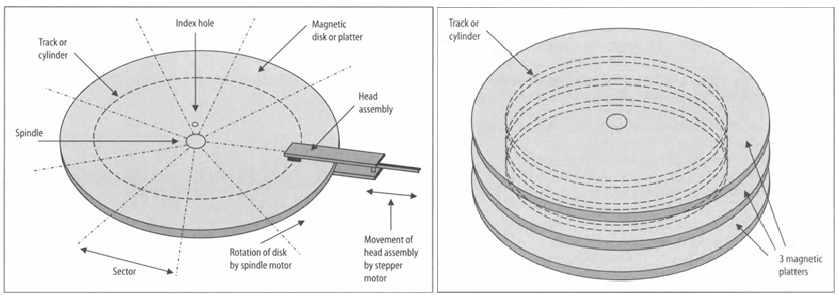
\includegraphics[width=0.95\textwidth]{resources/chapter-2/disk-structure.png}
	\caption{Struktur HDD \parencite{sammes2000disk}}
	\label{fig:hdd-structure}
\end{figure}

HDD terdiri atas susunan piringan dan penunjuk seperti yang diilustrasikan pada Gambar \ref{fig:hdd-structure}. Untuk mengakses data, pertama kali HDD harus membenarkan posisi dari kepala penunjuk sampai berada pada \textit{track} yang sesuai, waktu yang diperlukan untuk melakukan hal ini disebut dengan \textit{seek time}. Setelah kepala penunjuk sudah ada pada posisi, piringan harus berputar sampai sektor yang diperlukan berselarasan dengan kepala penunjuk tersebut, waktu ini disebut dengan \textit{rotational latency}. Karena piringan berputar terus menerus, waktu yang dibutuhkan untuk mencapai sektor yang benar bergantung pada kecepatan dari piringan tersebut. Kecepatan ini diukur menggunakan satuan \textit{rotations per minute} (RPM). Pemindahan data baru dapat dilakukan setelah kepala ada pada posisi sektor yang benar. Jika data tidak bersifat kontinu atau tersebar pada sektor yang berbeda-beda, penyesuaian kepala penunjuk dapat menyebabkan penambahan \textit{seek time} dan \textit{rotational latency} sesuai lokasi sektor tersebut. Pelaksanaan \textit{request} juga dipengaruhi oleh algoritma \textit{disk scheduling} yang digunakan \parencite{arpaci2018operating}.

Teknologi lain yang digunakan sebagai sistem penyimpanan adalah \textit{solid-state drive} (SSD). SSD tidak memiliki bagian mekanikal layaknya HDD, tetapi dibuat dari transistor seperti memori dan prosesor. Latensi dari SSD yang menggunakan teknologi \textit{flash} tidak lagi terpengaruh oleh peletakan data pada modul. Latensi berasal dari waktu yang digunakan oleh \textit{controller}. Hal yang dilakukan oleh \textit{controller} antara lain memetakan data pada blok, memanfaatkan \textit{cache} pada SSD, melakukan \textit{wear-leveling} untuk menyebar penggunaan block agar modul bertahan lebih lama, dan membersihkan dari blok yang sudah tidak terpakai. Dibandingkan dengan HDD, SSD memiliki kinerja yang jauh lebih baik dengan \textit{throughput} yang lebih tinggi dan latensi yang lebih rendah \parencite{arpaci2018operating}.

\subsection{Latensi Jaringan}

Latensi jaringan adalah waktu yang dibutuhkan untuk data menempuh jarak dari satu titik ke titik lainnya melewati jaringan. Secara teori, data dapat melintasi internet dengan kecepatan yang mendekati kecepatan cahaya. Namun, pada nyatanya, data bergerak lebih lambat sebab jarak, infrastruktur internet, ukuran paket, kemacetan jaringan, dan variabel lainnya \parencite{goodwin2023latency}. Hal ini terjadi ketika data perlu dikirim dari satu perangkat ke perangkat lainnya, misalnya pada aplikasi \textit{server} dan \textit{client}.

Pada sistem terdistribusi, latensi jaringa berperan besar terhadap \textit{response time} karena sistem terpisah dari lokasi fisik yang jauh. Hal ini disebabkan mendistribusikan data pada jaringan lokal tidak memiliki banyak guna \parencite{johansson2000impact}. Sekalipun berjarak dekat, pengiriman data antar perangkat membutuhkan waktu untuk mengirimkan data atau \textit{transmit time} dan penerimaan dari data tersebut di sisi penerima.

\subsection{Faktor Lain}


\section{\textit{Key-value Store Database}}

\subsection{\textit{In-memory Cache}}


\subsection{LSM-Tree}

\subsection{\textit{Direct SSD Access}}
\label{sec:direct-ssd-access}


\section{Sistem Terdistribusi}
\label{sec:sistem-terdistribusi}

Sistem terdistribusi adalah sistem yang terdiri dari lebih dari satu perangkat. 

\subsection{\textit{Consistency}}
\subsection{\textit{Availability}}
\subsection{\textit{Partition Tolerance}}

% ::NOTE: Are these relevant? Depends on the title, no?::
% \subsection{\textit{In-memory Cache}}


% \subsection{LSM-Tree}



\chapter{Analisis Persoalan dan Rancangan Solusi}
\label{chapter:analisis-persoalan-dan-rancangan-solusi}

Tujuan utama penulisan bab ini adalah untuk menjelaskan proses solusi atas masalah pencarian kondisi ketika \textit{erasure coding} memiliki \textit{response time} yang lebih cepat dibandingkan replikasi. Bagian ini memaparkan proses analisis masalah, rancangan solusi, serta implementasi solusi.

\section{Analisis}

Bagian ini menganalisis permasalahan lalu menurunkan kebutuhan sistem yang akan dibangun. Setelah itu, bagian ini juga membandingkan beberapa alternatif solusi yang dapat digunakan untuk menyelesaikan permasalahan tersebut.

\section{Analisis Permasalahan}
\label{sec:analisis-permasalahan}

% Berdasarkan latar belakang yang telah diuraikan pada \ref{sec:latar-belakang}, penggunaan \textit{erasure coding} pada sebuah sistem dapat mengurangi kebutuhan penyimpanan data dengan tetap menjaga integritas dan ketahanan data. Walaupun membutuhkan sumber daya komputasi dalam penerapannya, pengurangan ukuran data keseluruhan yang diperlukan menyebabkan juga turunnya ukuran data yang perlu dikirim ke \textit{node} lainnya.Hal ini menyebabkan mungkinnya terdapat suatu kondisi ketika {response time} yang diperlukan untuk melakukan operasi pada \textit{erasure coding} lebih rendah jika dibandingkan dengan melakukan operasi yang sama pada sistem yang menggunakan \textit{replikasi} untuk mencapai ketahanan tersebut.

Berdasarkan latar belakang dan studi literatur yang telah ditentukan, \textit{erasure coding} memiliki potensi untuk menghasilkan \textit{response time} yang lebih rendah dibandingkan dengan sistem berbasis \textit{replikasi} karena walaupun membutuhkan komputasi, ukuran data yang dikirimkan untuk ketahanan lebih rendah dibandingkan replikasi. Riset ini akan menganalisis faktor-faktor untuk mencapai kondisi tersebut. Faktor yang dianalisis antara lain ukuran data yang besar dan jaringan yang lambat. Dengan demikian, diperlukan sistem yang dapat mensimulasikan operasi pada sistem \textit{erasure coding} dan replikasi sekaligus memvariasikan faktor-faktor tersebut dalam operasinya tanpa memengaruhi kinerja sistem di sisi lain.

Dari permasalahan tersebut, dirumuskan kebutuhan sebuah perangkat lunak antara lain
\begin{enumerate}

    \item Sistem harus dapat mensimulasikan kondisi \textit{database} terdistribusi yang menggunakan replikasi ataupun \textit{erasure coding}.
    \item Sistem harus dapat menyimpan data secara \textit{persistent}.
    \item Sistem harus dapat memvariasikan ukuran data dan kecepatan jaringan.
    \item Sistem harus dapat menjalankan eksperimen berulang kali untuk mendapatkan data dari eksperimen.

\end{enumerate}

Penjelasan lebih detail mengenai kebutuhan sistem terdapat pada lampiran \ref{sec:rancangan-struktural}.
\subsection{Analisis Kebutuhan Sistem}
\label{sec:analisis-kebutuhan-sistem}

Berdasarkan bagian \ref{sec:analisis-permasalahan}, dirumuskan kebutuhan sebuah perangkat lunak antara lain
\begin{enumerate}

    \item Sistem harus dapat mensimulasikan kondisi \textit{database} terdistribusi yang menggunakan replikasi ataupun \textit{erasure coding}.
    \item Sistem harus dapat menyimpan data secara \textit{persistent} untuk mensimulasikan kegagalan dan pemulihan.
    \item Sistem harus dapat memvariasikan ukuran data, tingkat ketahanan, kecepatan jaringan, dan kemampuan komputasi.
    \item Sistem harus dapat menjalankan eksperimen berulang kali untuk mendapatkan data persentil dari eksperimen.

\end{enumerate}
\subsection{Alternatif Solusi}
\label{sec:alternatif-solusi}

Berdasarkan analisis permasalahan pada bagian \ref{sec:analisis-permasalahan} serta studi literatur, terdapat berbagai macam alternatif solusi untuk kebutuhan sistem tersebut.

\subsubsection{Menggunakan sistem Memcached gabungan dengan \textit{database} lain}
Pendekatan ini mengkombinasikan antara sistem \textit{in-memory key-value store} milik Memcache dan menggunakan \textit{database} terpisah sebagai tempat penyimpanan data \textit{persistence}. Replikasi dan \textit{erasure coding} dapat dilakukan pada data persisten yang disimpan pada \textit{database} tersebut. Kelebihan dari pendekatan ini adalah kemudahan dari implementasi dibandingkan pengembangan sendiri ataupun modifikasi \textit{database} yang sudah lebih kompleks. Namun, kekurangannya adalah \textit{overhead} penggunaan memori dari menjalankan Memcached dan \textit{database} terpisah. Dari ketiga alternatif solusi, kemudahan implementasi dan kekurangan yang dapat ditoleransi menjadikan alternatif ini solusi yang dipilih dalam penelitian ini.

\subsubsection{Menggunakan sistem Memcached dengan fitur-fitur yang dibutuhkan dikembangkan sendiri}
Pendekatan ini membangun fitur-fitur yang dibutuhkan untuk penelitian di atas Memcached secara mandiri. Kelebihan dari pendekatan ini kebebasan yang tinggi sehingga sistem dapat disesuaikan untuk eksperimen. Namun, pendekatan ini sulit mencerminkan kondisi nyata. Selain itu, kinerja sistem yang dikembangkan juga bergantung erat pada waktu serta kemampuan pengembangan peneliti.

\subsubsection{Mengembangkan sistem yang sudah memiliki fitur lengkap dengan mengganti \textit{source-code database} untuk fitur yang dibutuhkan}
Pengembangan ini membangun mengganti fitur yang dibutuhkan untuk penelitian di atas \textit{database} lebih kompleks dari Memcached. Pendekatan ini memiliki kelebihan kedekatan kondisi eksperimen dengan dunia nyata. Namun, pendekatan ini sulit dilakukan karena membutuhkan waktu yang lama untuk memahami dan mengubah \textit{source-code database} yang kompleks.


\section{Rancangan}
\label{sec:rancangan}

Bagian ini menjelaskan rancangan sistem yang akan diimplementasikan. Rancangan sistem merujuk pada kebutuhan sistem yang dihasilkan pada Bagian \ref{subsection:system-requirements} dan alternatif solusi yang dipilih pada Bagian \ref{subsection:alternatif-solusi}. Rancangan sistem ini mencakup struktur sistem, arsitektur sistem, alur transaksi, dan detail komponen yang akan diimplementasikan. Komponen didefinisikan sebagai sebuah unit fungsional yang berdiri sendiri dan dapat disusun.


\subsection{Rancangan Struktural}
\label{subsection:rancangan-struktural}

Seperti yang telah dijelaskan pada \ref{subsection:alternatif-solusi}, solusi yang dipilih adalah membuat sistem dengan mengkombinasikan \textit{in-memory key-value store} dan menggunakan RocksDB sebagai \textit{persistent database}. Replikasi dan \textit{erasure coding} hanya dilakukan pada data persisten yang disimpan pada \textit{database} tersebut sedangkan \textit{in-memory key-value store} berperan seperti \textit{cache} untuk meningkatkan kinerja sistem, khususnya untuk mengurangi rekonstruksi data dari \textit{persistent database} untuk \textit{erasure coding} pada operasi \textit{read}.

Mengikuti pendekatan pada \ref{subsubsection:pemilihan-pengembangan-sistem}, solusi dirancang untuk dibuat dalam bentuk komponen-komponen. Beberapa komponen disusun secara hierarkis dan membentuk subsistem yang mewakili domain tanggung jawab tertentu dalam sistem. Setiap komponen dirancang untuk memenuhi tujuan spesifik berdasarkan kebutuhan sistem.

\input{chapters/chapter-3/rancangan/01-01-node.tex}
\input{chapters/chapter-3/rancangan/01-02-data-collector.tex}
\subsection{Arsitektur Sistem}
\label{subsection:system-architecture}

Rancangan struktural yang telah dijelaskan pada Bagian \ref{subsection:rancangan-struktural} diimplementasikan sebagai sistem terdistribusi yang terdiri dari beberapa \textit{Node}. Komponen-komponen tersebut disusun dalam arsitektur sistem seperti yang ditunjukkan pada Gambar \ref{fig:general-architecture}.

Dalam gambaran umum arsitektur sistem, sistem \textit{Key-Value Store} terdistribusi yang dikembangkan adalah \textit{Node}. Dalam \textit{Node} terdapat komponen penyimpanan data yang dapat diakses dan dikelola secara terdistribusi dengan dapat replikasi atau \textit{erasure coding}. Setiap \textit{Node} dapat berkomunikasi dengan \textit{Node} lainnya untuk melakukan konsensus, replikasi data, dan pemulihan data.

Sementara itu, \textit{Data collector} merupakan \textit{script} eksternal yang tidak memiliki peran dalam sistem terdistribusi, namun berfungsi untuk mengumpulkan data eksperimen. Keterhubungan \textit{Data Collector} terbatas pada komponen \textit{benchmark} yang dapat mengatur konfigurasi dari sistem yang akan diujikan. Detail dari masing-masing komponen akan dijelaskan pada Bagian \ref{subsection:detail-komponen}. Ilustrasi keseluruhan arsitektur sistem yang memuat semua detail dapat dilihat pada Bagian \ref{appendix:detailed-architecture}.

\begin{figure}[ht]
	\centering
	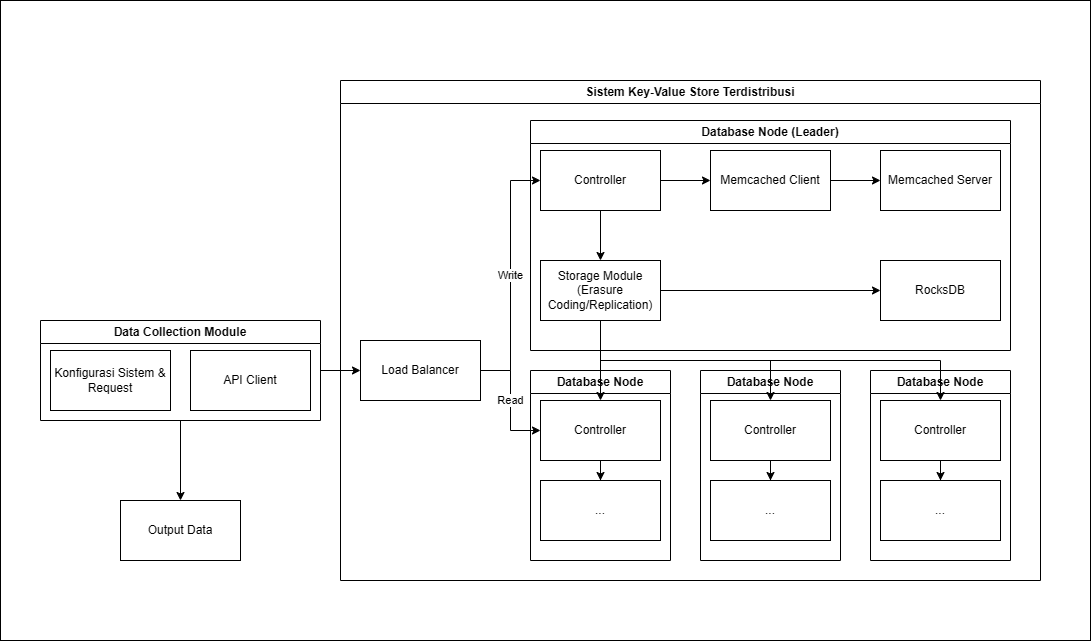
\includegraphics[width=0.75\textwidth]{resources/chapter-3/general-architecture.png}
	\caption{Gambaran Arsitektur Sistem Eksperimen}
	\label{fig:general-architecture}
\end{figure}

% Arsitektur dari sistem mengasumsikan kebutuhan untuk konsistensi yang tinggi. Untuk mencapai konsistensi tersebut, operasi \textit{write} dilakukan secara \textit{synchronous} dengan distribusi replikasi dan \textit{erasure coding} dianggap selesai ketika nilai ketahanan yang diinginkan sudah tercapai.

% Karena sistem bersifat terdistribusi, maka diperlukan sebuah algoritma konsensus untuk mengelola konsistensi antar \textit{Node}. Algoritma konsensus yang digunakan algoritma konsensus \textit{paxos} yang disesuaikan dengan kebutuhan. Salah satu penyesuaian yang dilakukan adalah mengadopsi pola \textit{leader-follower} untuk memudahkan sinkronisasi data dan mempercepat transaksi. Dengan adanya leader, fase 1 dari algoritma \textit{paxos} dapat dihilangkan dengan membuat proposal dari leader selalu memiliki nilai paling tinggi. Detail implementasi \textit{paxos} akan dijelaskan di Bagian \ref{subsection:detail-komponen}. Diagram gambaran arsitektur sistem dapat dilihat pada Gambar \ref{fig:general-architecture}.

% Operasi \textit{write} akan secara ekslusif disalurkan pada \textit{leader}. Kemudian untuk ketahanan, data akan didistribusikan pada \textit{follower} sesuai dengan konfigurasi \textit{node}. Sementara itu, operasi \textit{read} dapat dilakukan pada \textit{Node} manapun. Pada sistem \textit{erasure coding}, jika pada \textit{node} tersebut tidak terdapat nilai data yang dicari, maka \textit{Node} akan melakukan \textit{request} ke semua node lainnya untuk melakukan rekonstruksi data.

\subsection{Alur Transaksi}
\label{subsection:system-flow}

Mengikuti batasan pada Bagian \ref{sec:batasan-masalah}, transaksi yang akan diimplementasikan dalam sistem ini adalah transaksi \textit{write} dan \textit{read}. Sistem akan mendukung dua skema penyimpanan, yaitu replikasi dan \textit{erasure coding}, yang akan mempengaruhi alur transaksi.

\begin{figure}[!ht]
	\centering
	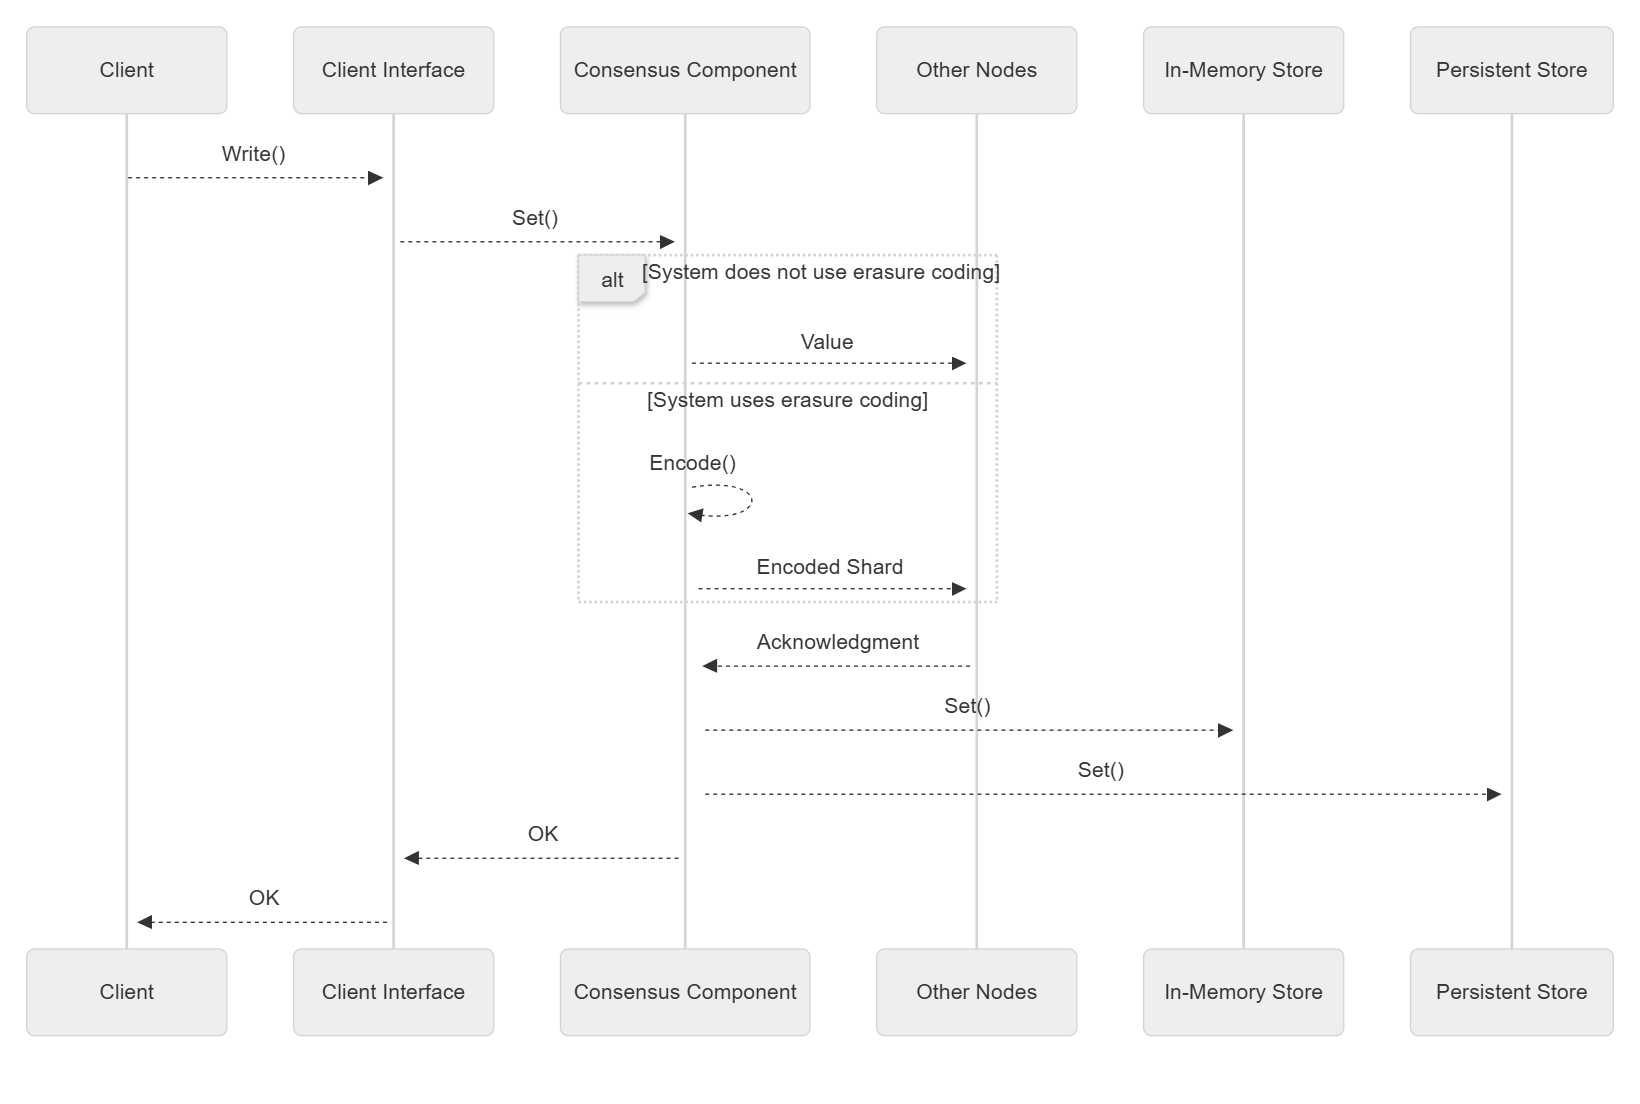
\includegraphics[width=0.95\textwidth]{resources/chapter-3/flow-write.png}
	\caption{Flow operasi \textit{write} dalam rancangan implementasi}
	\label{fig:flow-write-mermaidjs}
\end{figure}

Alur untuk transaksi \textit{write} dapat dilihat pada Gambar \ref{fig:flow-write-mermaidjs} dengan \textit{request} masuk ke \textit{Node}. Node kemudian akan melakukan operasi \textit{erasure coding} lalu menyebarkan \textit{shard} ke \textit{Node} lain sesuai dengan algoritma konsensus yang digunakan. Operasi \textit{write} dianggap selesai setelah konsensus mencapai kuorum.

\begin{figure}[!ht]
	\centering
	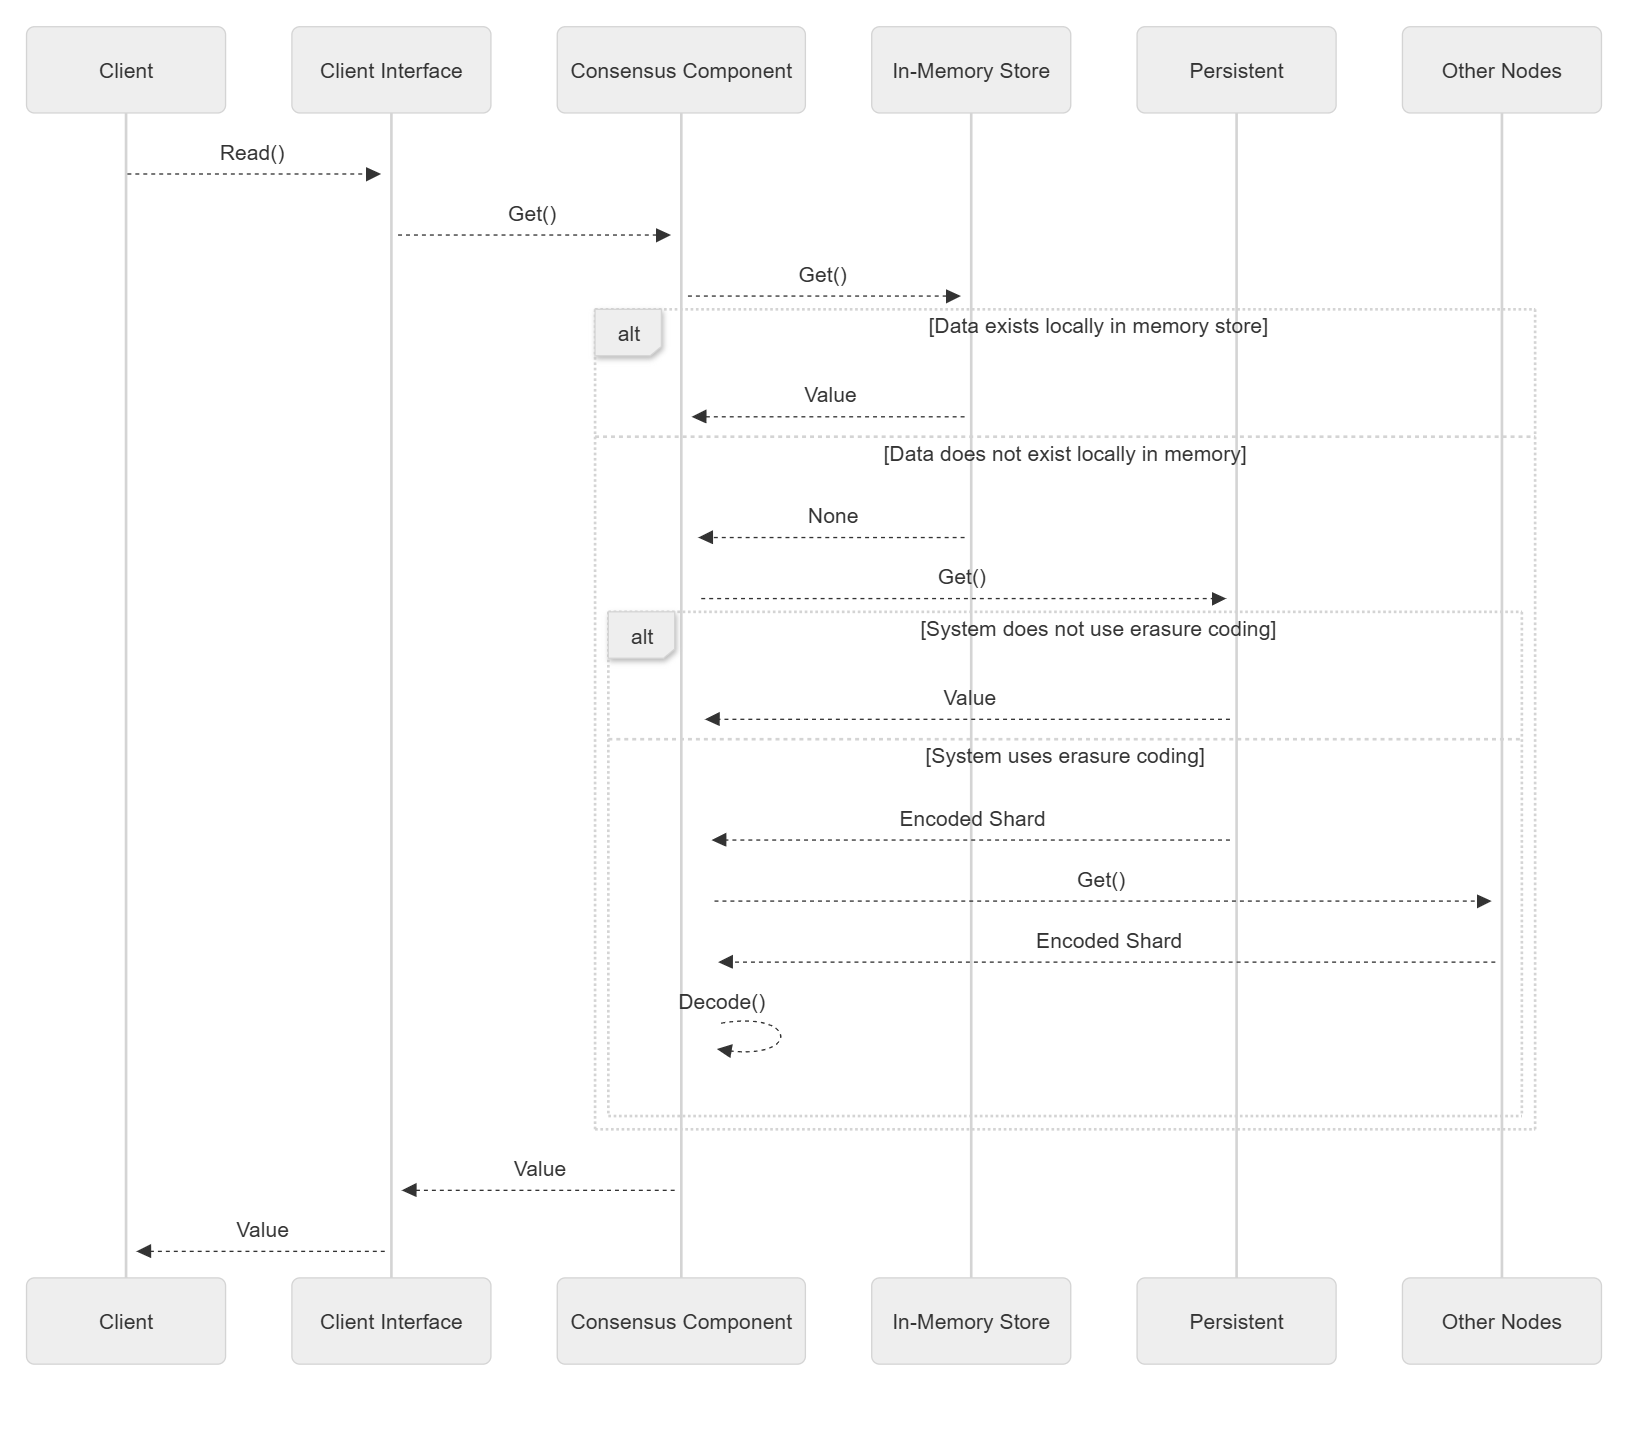
\includegraphics[width=0.95\textwidth]{resources/chapter-3/flow-read.png}
	\caption{Flow operasi \textit{read} dalam rancangan implementasi}
	\label{fig:flow-read-mermaidjs}
\end{figure}

Alur untuk transaksi \textit{read} dapat dilihat pada Gambar \ref{fig:flow-read-mermaidjs} dengan \textit{request} masuk ke \textit{Node} yang tersedia. \textit{node} melakukan operasi \textit{read} pada \textit{key-value store} dan mengembalikan hasil operasi ke \textit{client} jika tersedia. Jika tidak, maka \textit{Node} melakukan rekonstruksi data dari \textit{erasure-coded persistent data} yang tersebar pada \textit{node-node} lainnya. Pada replikasi, data diambil dari \textit{Node} lain yang memiliki data yang sama.
\subsection{Rancangan Detail Komponen}
\label{subsection:detail-komponen}

Berdasarkan rancangan struktural yang sudah dijelaskan pada bagian \ref{subsection:rancangan-struktural}, sistem akan diimplementasikan sebagai kumpulan komponen. Masing-masing komponen tersebut memiliki peran dan tanggung jawab yang berbeda dalam sistem eksperimen. Pada bagian ini, akan dijelaskan lebih lanjut mengenai rancangan detail dari masing-masing komponen tersebut.

\input{chapters/chapter-3/rancangan/04-01-detail-node.tex}
\input{chapters/chapter-3/rancangan/04-02-detail-konsensus.tex}
\input{chapters/chapter-3/rancangan/04-03-detail-client-interface.tex}
\input{chapters/chapter-3/rancangan/04-04-detail-internode-interface.tex}
\input{chapters/chapter-3/rancangan/04-05-detail-persistent-store.tex}
\input{chapters/chapter-3/rancangan/04-06-detail-memory-store.tex}
\input{chapters/chapter-3/rancangan/04-07-detail-data-collector.tex}
\input{chapters/chapter-3/rancangan/04-08-detail-testing.tex}
\input{chapters/chapter-3/rancangan/04-09-detail-logging.tex}


% \chapter{Evaluasi}
\label{chapter:Evaluasi}
Bab ini akan memaparkan evaluasi dari implementasi yang dilakukan beserta hasil analisis uji coba yang dilakukan. Tujuannya sebagai memberikan hasil utama dari penelitian tugas akhir ini.

::TODO::

% \section{Jadwal Pelaksanaan}
\label{sec:jadwal-pelaksanaan}
Aktivitas-aktivitas yang akan dilakukan untuk memenuhi kebutuhan eksperiman adalah seperti yang dapat dilihat pada tabel \ref{tab:rincian-aktivitas}.

\begin{table}[ht]
\centering
\caption{Daftar Aktivitas Tugas Akhir}
\begin{tabular}{|p{1cm}|p{6cm}|p{6cm}|}
\hline
\rowcolor{black!10} ID & Kegiatan & Hasil \\ \hline
K-1  & Melakukkan kajian pustaka & Bab II pada proposal tugas akhir \\ \hline
K-2  & Melakukan analisis permasalahan untuk topik tugas akhir & Bab I pada proposal tugas akhir \\ \hline
K-3  & Merancang solusi penyelesaian masalah & Bab III dan Bab IV pada proposal tugas akhir \\ \hline
K-4  & Melakukan finalisasi proposal tugas akhir & Proposal tugas akhir \\ \hline
K-5  & Melakukan seminar proposal tugas akhir & - \\ \hline
K-6  & Melakukan implementasi sistem \textit{key-value store database} untuk membandingkan \textit{erasure coding} dengan replikasi \textit{} & Sistem \textit{key-value store database} yang dapat mengumpulkan data untuk perbandingan \textit{erasure coding} dan replikasi \\ \hline
K-7  & Melakukan eksperimen untuk pengumpulan data \textit{response time} operasi pada sistem \textit{erasure coding} dan replikasi yang divariasikan sesuai rancangan & Data \textit{response time} operasi pada sistem \textit{erasure coding} dan replikasi \\ \hline
K-8  & Melakukan analisis data eksperimen & Hasil analisis \\ \hline
K-9  & Menyusun laporan tugas akhir secara keseluruhan & Laporan tugas akhir \\ \hline
K-10  & Melakukan sidang tugas akhir & - \\ \hline
\end{tabular}
\label{tab:rincian-aktivitas}
\end{table}

Dari aktivitas-aktivitas tersebut, jadwal perencanaan pelaksanaan masing-masing aktivitas dapat dilihat pada tabel \ref{tab:jadwal-part1} dan \ref{tab:jadwal-part2}.

\begin{table}[ht]
\centering
\caption{Jadwal Tugas Akhir Periode Oktober 2024 hingga Februari 2025}
\resizebox{\textwidth}{!}{
\begin{ganttchart}[
    title/.append style={fill=black!10},
    time slot format=simple,
    x unit=0.9cm,
    y unit chart=0.7cm,
    hgrid,
    vgrid
    ]{1}{20}

    \gantttitle{2024}{12}
    \gantttitle{2025}{8} \\

    \gantttitle{Oktober}{4}
    \gantttitle{November}{4}
    \gantttitle{Desember}{4}
    \gantttitle{Januari}{4}
    \gantttitle{Februari}{4}\\
    
    \gantttitle{14}{1}
    \gantttitle{21}{1}
    \gantttitle{28}{1}
    \gantttitle{4}{1}
    \gantttitle{11}{1}
    \gantttitle{18}{1}
    \gantttitle{25}{1} 
    \gantttitle{2}{1}
    \gantttitle{9}{1}
    \gantttitle{16}{1}
    \gantttitle{23}{1}
    \gantttitle{30}{1}
    \gantttitle{6}{1}
    \gantttitle{13}{1}
    \gantttitle{20}{1}
    \gantttitle{27}{1}
    \gantttitle{3}{1}
    \gantttitle{10}{1}
    \gantttitle{17}{1}
    \gantttitle{24}{1}\\

    \ganttbar{K-1}{1}{4} \\
    \ganttbar{K-2}{5}{6} \\
    \ganttbar{K-3}{7}{12} \\
    \ganttbar{K-4}{12}{13} \\
    \ganttbar{K-5}{14}{16} \\

\end{ganttchart}
}
\label{tab:jadwal-part1}
\centering
\caption{Jadwal Tugas Akhir Periode Maret 2025 hingga Juni 2025}
\resizebox{\textwidth}{!}{
\begin{ganttchart}[
    title/.append style={fill=black!10},
    time slot format=simple,
    x unit=0.9cm,
    y unit chart=0.7cm,
    hgrid,
    vgrid
    ]{1}{17}

    \gantttitle{2025}{17} \\

    \gantttitle{Maret}{5}
    \gantttitle{April}{4}
    \gantttitle{Mei}{4}
    \gantttitle{Juni}{4}\\
    
    \gantttitle{3}{1}
    \gantttitle{10}{1}
    \gantttitle{17}{1}
    \gantttitle{24}{1}
    \gantttitle{31}{1}
    \gantttitle{7}{1}
    \gantttitle{14}{1} 
    \gantttitle{21}{1}
    \gantttitle{28}{1}
    \gantttitle{5}{1}
    \gantttitle{12}{1}
    \gantttitle{19}{1}
    \gantttitle{26}{1}
    \gantttitle{2}{1}
    \gantttitle{9}{1}
    \gantttitle{16}{1}
    \gantttitle{23}{1}\\

    \ganttbar{K-6}{1}{4} \\
    \ganttbar{K-7}{5}{6} \\
    \ganttbar{K-8}{7}{12} \\
    \ganttbar{K-9}{12}{13} \\
    \ganttbar{K-10}{14}{16} \\

\end{ganttchart}
}
\label{tab:jadwal-part2}
\end{table}




% \section{Risiko Pelaksanaan}
\label{sec:risiko-pelaksanaan}
Berikut risiko yang mungkin dihadapi dalam pelaksanaan penelitian ini beserta rencana mitigasinya:

\begin{enumerate}
    \item Kompleksitas dalam implementasi dapat menghambat pelaksanaan penelitian ataupun memperburuk data untuk analisis dengan memberikan kebutuhan komputasi yang tidak selayaknya. Hal yang dapat dilakukan untuk menurunkan kompleksitas dalam implementasi adalah dengan menggunakan pustaka yang matang bila memungkinkan. Selain itu, bisa juga dilakukan validasi awal pada implementasi yang lebih sederhana untuk memastikan implementasi berfungsi sesuai kebutuhan sebelum diterapkan secara penuh.
    \item Risiko lain yang perlu dipertimbangkan adalah untuk memvariasikan kecepatan komputasi. Hal ini memerlukan penggunaan perangkat keras yang berbeda-beda. Mitigasi yang dilakukan adalah dengan menggunakan \textit{credit} pemberian platform \textit{cloud computing}. Jika masih tidak memungkinkan, penggunaan \textit{virtual machine} lokal dengan alokasi \textit{resource} yang disesuaikan.
    \item Kesalahan analisis hasil dapat terjadi jika terdapat kesalahan interpretasi hasil. Mitigasi yang dilakukan adalah dengan melakukan validasi dan menggunakan analisis statistik yang valid. Misalnya penggunaan \textit{percentile} yang lebih tahan terhadap \textit{outlier} dibandingkan dengan \textit{mean}.
    \item Kesalahan analisis juga dapat terjadi jika ada kesalahan dalam konfigurasi yang diguakan untuk perbandingan. Perbandingan \textit{erasure coding} dan replikasi memerlukan konfigurasi yang sama dan perbedaan konfigurasi dapat memengaruhi hasil penelitian. Cara untuk mencegah hal ini terjadi adalah dengan menentukan konfigurasi yang seragam dan terdokumentasi dengan jelas ketika penelitian berlangsung.
\end{enumerate}


% \chapter{Penutup}
\label{chapter:penutup}
Bagian akhir dari penelitian ini akan membahas kesimpulan dan saran yang dapat diberikan berdasarkan hasil penelitian yang telah dilakukan. Kesimpulan akan merangkum hasil utama dari penelitian ini serta ketercapaian tujuan penelitian tugas akhir. Selain itu, saran akan memberikan rekomendasi untuk penelitian selanjutnya atau pengembangan sistem yang telah dibangun.

\section{Kesimpulan}
\label{sec:kesimpulan}
\section{Saran}
\label{sec:saran}

Adapun banyak kekurangan dari penelitian ini yang dapat diperbaiki pada penelitian selanjutnya. Beberapa saran yang dapat diberikan untuk penelitian selanjutnya adalah sebagai berikut:

\begin{enumerate}
	\item Penilitian ini tidak mencakup analisis proses \textit{recovery} dari \textit{erasure coding} yang dilakukan ketika terjadi kehilangan data. Perubahan konsensus yang dilakukan dengan adanya proses \textit{erasure coding} dapat mempengaruhi \textit{consistency} dan \textit{availability} dari \textit{database} terdistribusi.
	\item Penilitian ini tidak mencakup keseluruhan variabel yang dapat mempengaruhi kinerja sistem \textit{erasure coding} dan replikasi. Dapat dilakukan penelitian lebih lanjut untuk variasi dari konfigurasi sistem atau percobaan menggunakan beberapa sistem berbeda untuk mensimulasikan perbedaan kinerja.
	\item Pengembangan sistem \textit{hybrid} yang menggabungkan \textit{erasure coding} dan replikasi seperti disarankan untuk melakukan penelitian lanjutan yang menganalisis kinerja sistem. Penggabungan ini berpotensi memberikan solusi dengan keunggulan kedua sistem \textit{erasure coding} dan replikasi. Sistem \textit{hybrid} dapat digunakan misalnya dengan menggunakan replikasi untuk data yang sering dibaca atau berukuran kecil dan menggunakan \textit{erasure coding} untuk data yang bersifat arsip, jarang diakses, berukuran besar, atau pada beban kerja yang didominasi operasi \textit{write}.
	\item Optimasi dapat dilakukan untuk meningkatkan kinerja \textit{erasure coding}. Implementasi \textit{erasure coding} yang digunakan pada penelitian ini adalah implementasi sederhana. Salah satu optimasi adalah penambahan berupa \textit{worker} yang melakukan algoritma \textit{encoding} atau \textit{decoding} secara paralel dapat meningkatkan kinerja \textit{erasure coding}.
	\item Penelitian ini tidak mencakup percobaan sistem nyata dengan jarak geografis serta variasi dari sistem yang digunakan. Hal ini berpotensi memberikan hasil yang berbeda dengan percobaan yang dilakukan pada penelitian ini.
\end{enumerate}

%---------------------------------------------------------------%

% Daftar pustaka
\printbibliography{}

% Setting judul lampiran
\titlespacing*{\chapter}{0pt}{0pt}{0pt}
\titlespacing*{\section}{0pt}{0pt}{*1}

% Setting judul anak lampiran
\titleformat*{\section}{\bfseries}

% \appendix

\chapter{Detail Arsitektur Sistem}
\label{appendix:detailed-architecture}

Gambar \ref{fig:detailed-architecture} menunjukkan gambaran detail arsitektur sistem eksperimen yang digunakan dalam penelitian ini. Arsitektur ini mencakup komponen-komponen utama yang berperan dalam pengumpulan data, pengelolaan konsistensi, dan replikasi data antar \textit{Node} seperti yang telah dijelaskan pada Bagian \ref{sec:rancangan}

\begin{figure}[ht]
    \centering
    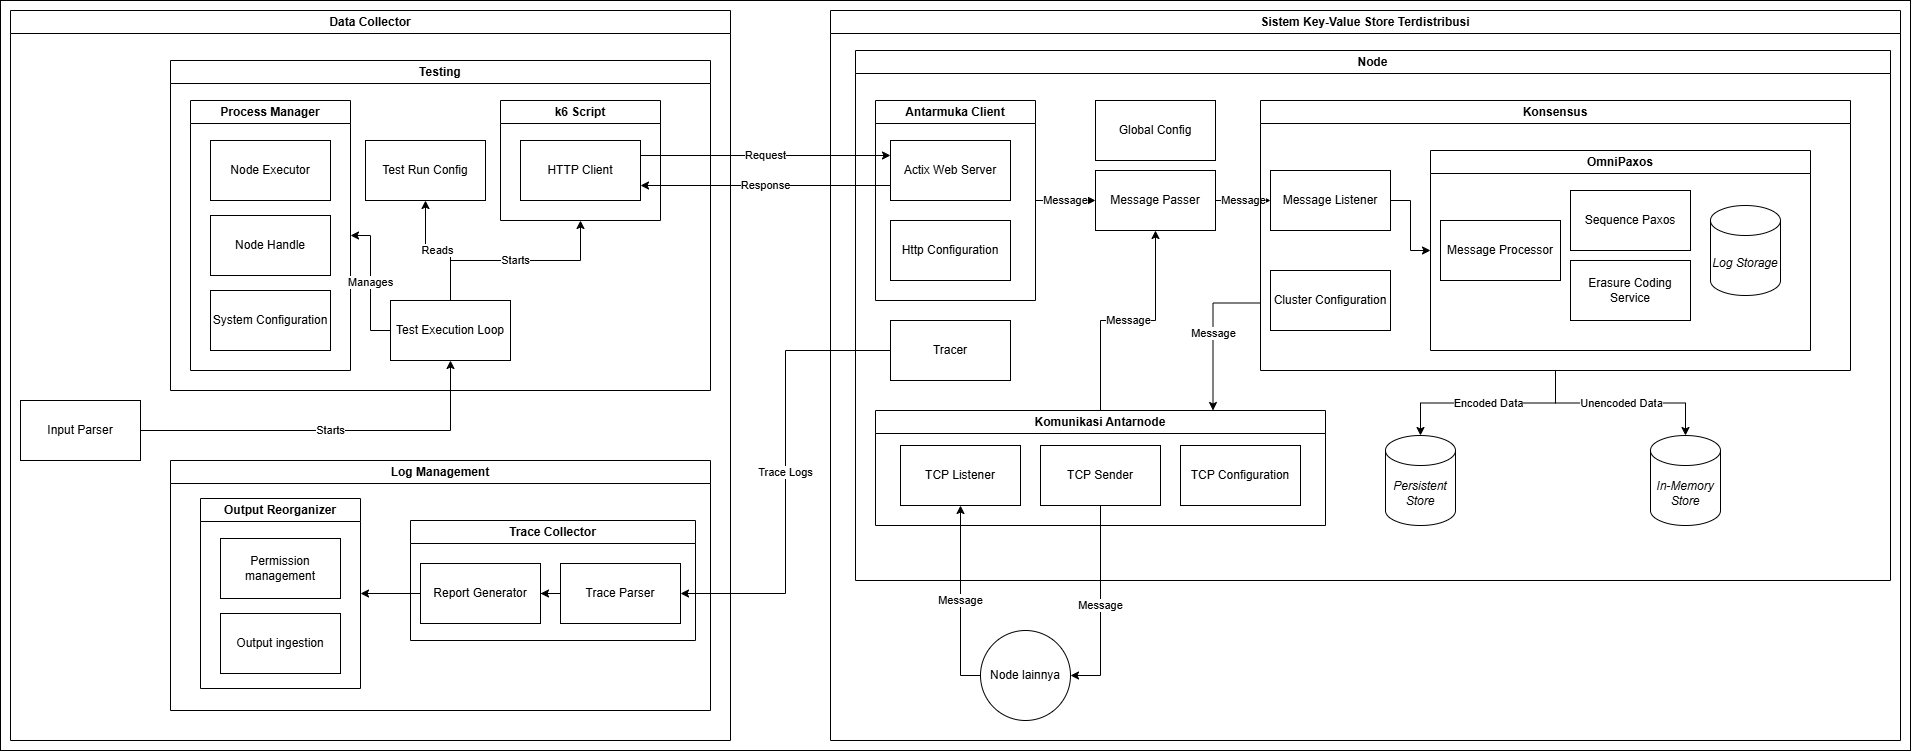
\includegraphics[width=\textwidth]{resources/appendix/detailed-architecture.png}
    
    \caption{Gambaran Detail Arsitektur Sistem Eksperimen}
    \label{fig:detailed-architecture}
\end{figure}
\chapter{Pemetaan Pengujian}
\label{appendix:pemetaan-pengujian}

Lampiran ini menyediakan tabel yang memetakan kebutuhan fungsional dan non-fungsional ke pengujian yang dilakukan. Tujuannya adalah memudahkan pemetaan antara kebutuhan sistem dan pengujian yang dilakukan serta memastikan bahwa semua kebutuhan telah diuji.

\begin{longtable}{|l|l|p{3cm}|p{3cm}|l|}
\caption{Pemetaan Pengujian}
\label{tab:pemetaan-pengujian} \\
\hline
\rowcolor{black!10} ID Kebutuhan & ID Pengujian & Skenario & Ekspektasi & Realita \\ \hline
\endfirsthead

\caption[]{Pemetaan Pengujian (lanjutan)} \\
\hline
\rowcolor{black!10} ID Kebutuhan & ID Pengujian & Skenario & Ekspektasi & Realita \\ \hline
\endhead

F-1 & P-1 & Pengujian operasi \textit{write} pada sistem & Sistem dapat menyimpan \textit{key-value pair} menggunakan operasi \textit{write} & Sesuai \\ \hline
F-1 & P-2 & Pengujian operasi \textit{read} pada sistem & Nilai \textit{value} dapat didapatkan menggunakan operasi \textit{read} & Sesuai \\ \hline
F-2 & P-3 & Pengujian penyimpanan data \textit{persistent} & Sistem dapat menyimpan data secara \textit{persistent} & Sesuai \\ \hline
\end{longtable}

\end{document}
